% Options for packages loaded elsewhere
\PassOptionsToPackage{unicode}{hyperref}
\PassOptionsToPackage{hyphens}{url}
%
\documentclass[
  english,
  ignorenonframetext,
]{beamer}
\title{Estrategias Transversales en las Encuestas de Hogares}
\subtitle{Curso de Muestreo Probabilístico en Encuestas de Hogares}
\author{Andrés Gutiérrez, Ph.D.}
\date{CEPAL - Unidad de Estadísticas Sociales}

\usepackage{pgfpages}
\setbeamertemplate{caption}[numbered]
\setbeamertemplate{caption label separator}{: }
\setbeamercolor{caption name}{fg=normal text.fg}
\beamertemplatenavigationsymbolsempty
% Prevent slide breaks in the middle of a paragraph
\widowpenalties 1 10000
\raggedbottom
\setbeamertemplate{part page}{
  \centering
  \begin{beamercolorbox}[sep=16pt,center]{part title}
    \usebeamerfont{part title}\insertpart\par
  \end{beamercolorbox}
}
\setbeamertemplate{section page}{
  \centering
  \begin{beamercolorbox}[sep=12pt,center]{part title}
    \usebeamerfont{section title}\insertsection\par
  \end{beamercolorbox}
}
\setbeamertemplate{subsection page}{
  \centering
  \begin{beamercolorbox}[sep=8pt,center]{part title}
    \usebeamerfont{subsection title}\insertsubsection\par
  \end{beamercolorbox}
}
\AtBeginPart{
  \frame{\partpage}
}
\AtBeginSection{
  \ifbibliography
  \else
    \frame{\sectionpage}
  \fi
}
\AtBeginSubsection{
  \frame{\subsectionpage}
}
\usepackage{amsmath,amssymb}
\usepackage{lmodern}
\usepackage{iftex}
\ifPDFTeX
  \usepackage[T1]{fontenc}
  \usepackage[utf8]{inputenc}
  \usepackage{textcomp} % provide euro and other symbols
\else % if luatex or xetex
  \usepackage{unicode-math}
  \defaultfontfeatures{Scale=MatchLowercase}
  \defaultfontfeatures[\rmfamily]{Ligatures=TeX,Scale=1}
\fi
\usetheme[]{Pittsburgh}
% Use upquote if available, for straight quotes in verbatim environments
\IfFileExists{upquote.sty}{\usepackage{upquote}}{}
\IfFileExists{microtype.sty}{% use microtype if available
  \usepackage[]{microtype}
  \UseMicrotypeSet[protrusion]{basicmath} % disable protrusion for tt fonts
}{}
\makeatletter
\@ifundefined{KOMAClassName}{% if non-KOMA class
  \IfFileExists{parskip.sty}{%
    \usepackage{parskip}
  }{% else
    \setlength{\parindent}{0pt}
    \setlength{\parskip}{6pt plus 2pt minus 1pt}}
}{% if KOMA class
  \KOMAoptions{parskip=half}}
\makeatother
\usepackage{xcolor}
\IfFileExists{xurl.sty}{\usepackage{xurl}}{} % add URL line breaks if available
\IfFileExists{bookmark.sty}{\usepackage{bookmark}}{\usepackage{hyperref}}
\hypersetup{
  pdftitle={Estrategias Transversales en las Encuestas de Hogares},
  pdfauthor={Andrés Gutiérrez, Ph.D.},
  pdflang={en},
  hidelinks,
  pdfcreator={LaTeX via pandoc}}
\urlstyle{same} % disable monospaced font for URLs
\newif\ifbibliography
\usepackage{color}
\usepackage{fancyvrb}
\newcommand{\VerbBar}{|}
\newcommand{\VERB}{\Verb[commandchars=\\\{\}]}
\DefineVerbatimEnvironment{Highlighting}{Verbatim}{commandchars=\\\{\}}
% Add ',fontsize=\small' for more characters per line
\usepackage{framed}
\definecolor{shadecolor}{RGB}{248,248,248}
\newenvironment{Shaded}{\begin{snugshade}}{\end{snugshade}}
\newcommand{\AlertTok}[1]{\textcolor[rgb]{0.94,0.16,0.16}{#1}}
\newcommand{\AnnotationTok}[1]{\textcolor[rgb]{0.56,0.35,0.01}{\textbf{\textit{#1}}}}
\newcommand{\AttributeTok}[1]{\textcolor[rgb]{0.77,0.63,0.00}{#1}}
\newcommand{\BaseNTok}[1]{\textcolor[rgb]{0.00,0.00,0.81}{#1}}
\newcommand{\BuiltInTok}[1]{#1}
\newcommand{\CharTok}[1]{\textcolor[rgb]{0.31,0.60,0.02}{#1}}
\newcommand{\CommentTok}[1]{\textcolor[rgb]{0.56,0.35,0.01}{\textit{#1}}}
\newcommand{\CommentVarTok}[1]{\textcolor[rgb]{0.56,0.35,0.01}{\textbf{\textit{#1}}}}
\newcommand{\ConstantTok}[1]{\textcolor[rgb]{0.00,0.00,0.00}{#1}}
\newcommand{\ControlFlowTok}[1]{\textcolor[rgb]{0.13,0.29,0.53}{\textbf{#1}}}
\newcommand{\DataTypeTok}[1]{\textcolor[rgb]{0.13,0.29,0.53}{#1}}
\newcommand{\DecValTok}[1]{\textcolor[rgb]{0.00,0.00,0.81}{#1}}
\newcommand{\DocumentationTok}[1]{\textcolor[rgb]{0.56,0.35,0.01}{\textbf{\textit{#1}}}}
\newcommand{\ErrorTok}[1]{\textcolor[rgb]{0.64,0.00,0.00}{\textbf{#1}}}
\newcommand{\ExtensionTok}[1]{#1}
\newcommand{\FloatTok}[1]{\textcolor[rgb]{0.00,0.00,0.81}{#1}}
\newcommand{\FunctionTok}[1]{\textcolor[rgb]{0.00,0.00,0.00}{#1}}
\newcommand{\ImportTok}[1]{#1}
\newcommand{\InformationTok}[1]{\textcolor[rgb]{0.56,0.35,0.01}{\textbf{\textit{#1}}}}
\newcommand{\KeywordTok}[1]{\textcolor[rgb]{0.13,0.29,0.53}{\textbf{#1}}}
\newcommand{\NormalTok}[1]{#1}
\newcommand{\OperatorTok}[1]{\textcolor[rgb]{0.81,0.36,0.00}{\textbf{#1}}}
\newcommand{\OtherTok}[1]{\textcolor[rgb]{0.56,0.35,0.01}{#1}}
\newcommand{\PreprocessorTok}[1]{\textcolor[rgb]{0.56,0.35,0.01}{\textit{#1}}}
\newcommand{\RegionMarkerTok}[1]{#1}
\newcommand{\SpecialCharTok}[1]{\textcolor[rgb]{0.00,0.00,0.00}{#1}}
\newcommand{\SpecialStringTok}[1]{\textcolor[rgb]{0.31,0.60,0.02}{#1}}
\newcommand{\StringTok}[1]{\textcolor[rgb]{0.31,0.60,0.02}{#1}}
\newcommand{\VariableTok}[1]{\textcolor[rgb]{0.00,0.00,0.00}{#1}}
\newcommand{\VerbatimStringTok}[1]{\textcolor[rgb]{0.31,0.60,0.02}{#1}}
\newcommand{\WarningTok}[1]{\textcolor[rgb]{0.56,0.35,0.01}{\textbf{\textit{#1}}}}
\usepackage{longtable,booktabs,array}
\usepackage{calc} % for calculating minipage widths
\usepackage{caption}
% Make caption package work with longtable
\makeatletter
\def\fnum@table{\tablename~\thetable}
\makeatother
\usepackage{graphicx}
\makeatletter
\def\maxwidth{\ifdim\Gin@nat@width>\linewidth\linewidth\else\Gin@nat@width\fi}
\def\maxheight{\ifdim\Gin@nat@height>\textheight\textheight\else\Gin@nat@height\fi}
\makeatother
% Scale images if necessary, so that they will not overflow the page
% margins by default, and it is still possible to overwrite the defaults
% using explicit options in \includegraphics[width, height, ...]{}
\setkeys{Gin}{width=\maxwidth,height=\maxheight,keepaspectratio}
% Set default figure placement to htbp
\makeatletter
\def\fps@figure{htbp}
\makeatother
\setlength{\emergencystretch}{3em} % prevent overfull lines
\providecommand{\tightlist}{%
  \setlength{\itemsep}{0pt}\setlength{\parskip}{0pt}}
\setcounter{secnumdepth}{-\maxdimen} % remove section numbering
\usepackage{graphicx}
\usepackage{verbatim}
\ifXeTeX
  % Load polyglossia as late as possible: uses bidi with RTL langages (e.g. Hebrew, Arabic)
  \usepackage{polyglossia}
  \setmainlanguage[]{english}
\else
  \usepackage[main=english]{babel}
% get rid of language-specific shorthands (see #6817):
\let\LanguageShortHands\languageshorthands
\def\languageshorthands#1{}
\fi
\ifLuaTeX
  \usepackage{selnolig}  % disable illegal ligatures
\fi

\begin{document}
\frame{\titlepage}

\begin{frame}[allowframebreaks]
  \tableofcontents[hideallsubsections]
\end{frame}
\begin{frame}{Motivación}
\protect\hypertarget{motivaciuxf3n}{}
\begin{quote}
Desde que se popularizaron las encuestas de hogares en 1940, se ha hecho
evidente algunas tendencias que están ligadas a los avances tecnológicos
en las agencias estadísticas y en la sociedad y se han acelerado con la
introducción del computador.
\end{quote}

Gambino \& Silva (2009)
\end{frame}

\begin{frame}[fragile]{Bibliografía y referencias}
\protect\hypertarget{bibliografuxeda-y-referencias}{}
\begin{itemize}
\tightlist
\item
  Kish, L. (1965) \emph{Survey Sampling}. John Wiley and Sons.
\item
  Cochran, W. G. (1977) \emph{Sampling Techniques}. John Wiley and Sons.
\item
  Särndal, et. al.~(2003) \emph{Model-assisted Survey Sampling}.
  Springer.
\item
  Gutiérrez, H. A. (2016) \emph{Estrategias de muestreo: diseño de
  encuestas y estimación de parámetros}. Ediciones de la U.
\item
  Gutiérrez, H. A. (2017) \texttt{TeachingSampling}. \emph{R package}.
\end{itemize}
\end{frame}

\hypertarget{muestreo-aleatorio-simple-en-dos-etapas-estratificado}{%
\section{Muestreo aleatorio simple en dos etapas
estratificado}\label{muestreo-aleatorio-simple-en-dos-etapas-estratificado}}

\begin{frame}{Muestreo en dos etapas estratificado}
\protect\hypertarget{muestreo-en-dos-etapas-estratificado}{}
\begin{itemize}
\tightlist
\item
  La teoría discutida en las secciones anteriores es aplicable cuando
  las unidades primarias de muestreo son seleccionadas dentro de un
  estrato.
\item
  No hay nuevos principios de estimación o diseño involucrado en el
  desarrollo de esta estrategia de muestreo.
\end{itemize}
\end{frame}

\begin{frame}{Muestreo en dos etapas estratificado}
\protect\hypertarget{muestreo-en-dos-etapas-estratificado-1}{}
\begin{itemize}
\tightlist
\item
  Se supone que el muestreo en cada estrato respeta el principio de la
  independencia.
\item
  Las estimaciones del total, así como el cálculo y estimación de la
  varianza son simplemente resultado de añadir o sumar para cada estrato
  la respectiva cantidad.
\end{itemize}
\end{frame}

\begin{frame}{Muestreo en dos etapas estratificado}
\protect\hypertarget{muestreo-en-dos-etapas-estratificado-2}{}
\begin{itemize}
\tightlist
\item
  Dentro de cada estrato \(U_h\) \(h=1,\ldots, H\) existen \(N_{Ih}\)
  unidades primarias de muestreo, de las cuales se selecciona una
  muestra \(s_{Ih}\) de \(n_{Ih}\) unidades mediante un diseño de
  muestreo aleatorio simple.
\item
  Suponga, además que el sub-muestreo dentro de cada unidad primaria
  seleccionada es también aleatorio simple.
\item
  Para cada unidad primaria de muestreo seleccionada \(i\in s_{Ih}\) de
  tamaño \(N_i\) se selecciona una muestra \(s_i\) de elementos de
  tamaño \(n_i\).
\end{itemize}
\end{frame}

\begin{frame}{Muestreo en dos etapas estratificado}
\protect\hypertarget{muestreo-en-dos-etapas-estratificado-3}{}
Para utilizar los prinicpios de estimación del último conglomerado en
este diseño particular se definen las siguientes cantidades:

\begin{enumerate}
\tightlist
\item
  \(d_{I_i} = \dfrac{N_{Ih}}{n_{Ih}}\), que es el factor de expansión de
  la \(i\)-ésima UPM en el estrato \(h\).
\item
  \(d_{k|i} = \dfrac{N_{i}}{n_{i}}\), que es el factor de expansión del
  \(k\)-ésimo hogar para la \(i\)-ésima UPM.
\item
  \(d_k = d_{I_i} \times d_{k|i} = \dfrac{N_{Ih}}{n_{Ih}} \times \dfrac{N_{i}}{n_{i}}\),
  que es el factor de expansión final del \(k\)-ésimo elemento para toda
  la población \(U\).
\end{enumerate}
\end{frame}

\begin{frame}[fragile]{Práctica en \texttt{R}}
\protect\hypertarget{pruxe1ctica-en-r}{}
\begin{Shaded}
\begin{Highlighting}[]
\FunctionTok{data}\NormalTok{(}\StringTok{\textquotesingle{}BigCity\textquotesingle{}}\NormalTok{)}

\NormalTok{ FrameI }\OtherTok{\textless{}{-}}\NormalTok{ BigCity }\SpecialCharTok{\%\textgreater{}\%} \FunctionTok{group\_by}\NormalTok{(PSU) }\SpecialCharTok{\%\textgreater{}\%}
 \FunctionTok{summarise}\NormalTok{(}\AttributeTok{Stratum =} \FunctionTok{unique}\NormalTok{(Stratum),}
           \AttributeTok{Persons =} \FunctionTok{n}\NormalTok{(),}
           \AttributeTok{Income =} \FunctionTok{sum}\NormalTok{(Income),}
           \AttributeTok{Expenditure =} \FunctionTok{sum}\NormalTok{(Expenditure))}
             
\FunctionTok{attach}\NormalTok{(FrameI)}
\end{Highlighting}
\end{Shaded}
\end{frame}

\begin{frame}[fragile]{Práctica en \texttt{R}}
\protect\hypertarget{pruxe1ctica-en-r-1}{}
\begin{Shaded}
\begin{Highlighting}[]
\FunctionTok{head}\NormalTok{(FrameI, }\DecValTok{10}\NormalTok{)}
\end{Highlighting}
\end{Shaded}

\begin{longtable}[]{@{}llrrr@{}}
\toprule
PSU & Stratum & Persons & Income & Expenditure \\
\midrule
\endhead
PSU0001 & idStrt001 & 118 & 70912 & 44232 \\
PSU0002 & idStrt001 & 136 & 68887 & 38382 \\
PSU0003 & idStrt001 & 96 & 37213 & 19495 \\
PSU0004 & idStrt001 & 88 & 36926 & 24031 \\
PSU0005 & idStrt001 & 110 & 57494 & 31142 \\
PSU0006 & idStrt001 & 116 & 75272 & 43473 \\
PSU0007 & idStrt001 & 68 & 33028 & 21833 \\
PSU0008 & idStrt001 & 136 & 64293 & 47660 \\
PSU0009 & idStrt001 & 122 & 33156 & 23292 \\
PSU0010 & idStrt002 & 70 & 65254 & 37115 \\
\bottomrule
\end{longtable}
\end{frame}

\begin{frame}[fragile]{Práctica en \texttt{R}}
\protect\hypertarget{pruxe1ctica-en-r-2}{}
\begin{Shaded}
\begin{Highlighting}[]
\NormalTok{sizes }\OtherTok{=}\NormalTok{ FrameI }\SpecialCharTok{\%\textgreater{}\%} \FunctionTok{group\_by}\NormalTok{(Stratum) }\SpecialCharTok{\%\textgreater{}\%}
        \FunctionTok{summarise}\NormalTok{(}\AttributeTok{NIh =} \FunctionTok{n}\NormalTok{(),}
        \AttributeTok{nIh =} \DecValTok{2}\NormalTok{,}
        \AttributeTok{dI =}\NormalTok{ NIh}\SpecialCharTok{/}\NormalTok{nIh)}
        
\NormalTok{NIh }\OtherTok{\textless{}{-}}\NormalTok{ sizes}\SpecialCharTok{$}\NormalTok{NIh}
\NormalTok{nIh }\OtherTok{\textless{}{-}}\NormalTok{ sizes}\SpecialCharTok{$}\NormalTok{nIh}
\end{Highlighting}
\end{Shaded}
\end{frame}

\begin{frame}[fragile]{Práctica en \texttt{R}}
\protect\hypertarget{pruxe1ctica-en-r-3}{}
\begin{Shaded}
\begin{Highlighting}[]
\FunctionTok{head}\NormalTok{(sizes, }\DecValTok{10}\NormalTok{)}
\end{Highlighting}
\end{Shaded}

\begin{longtable}[]{@{}lrrr@{}}
\toprule
Stratum & NIh & nIh & dI \\
\midrule
\endhead
idStrt001 & 9 & 2 & 4.5 \\
idStrt002 & 11 & 2 & 5.5 \\
idStrt003 & 7 & 2 & 3.5 \\
idStrt004 & 13 & 2 & 6.5 \\
idStrt005 & 11 & 2 & 5.5 \\
idStrt006 & 5 & 2 & 2.5 \\
idStrt007 & 14 & 2 & 7.0 \\
idStrt008 & 7 & 2 & 3.5 \\
idStrt009 & 8 & 2 & 4.0 \\
idStrt010 & 8 & 2 & 4.0 \\
\bottomrule
\end{longtable}
\end{frame}

\begin{frame}[fragile]{Práctica en \texttt{R}}
\protect\hypertarget{pruxe1ctica-en-r-4}{}
\footnotesize

\begin{Shaded}
\begin{Highlighting}[]
\NormalTok{samI }\OtherTok{\textless{}{-}} \FunctionTok{S.STSI}\NormalTok{(Stratum, NIh, nIh)}
\NormalTok{UI }\OtherTok{\textless{}{-}} \FunctionTok{levels}\NormalTok{(}\FunctionTok{as.factor}\NormalTok{(FrameI}\SpecialCharTok{$}\NormalTok{PSU))}
\NormalTok{sampleI }\OtherTok{\textless{}{-}}\NormalTok{ UI[samI]}

\NormalTok{FrameII }\OtherTok{\textless{}{-}} \FunctionTok{left\_join}\NormalTok{(sizes, }
\NormalTok{            BigCity[}\FunctionTok{which}\NormalTok{(BigCity}\SpecialCharTok{$}\NormalTok{PSU }\SpecialCharTok{\%in\%}\NormalTok{ sampleI), ])}
\FunctionTok{attach}\NormalTok{(FrameII)}
\end{Highlighting}
\end{Shaded}
\end{frame}

\begin{frame}[fragile]{Práctica en \texttt{R}}
\protect\hypertarget{pruxe1ctica-en-r-5}{}
\begin{Shaded}
\begin{Highlighting}[]
\FunctionTok{head}\NormalTok{(FrameII, }\DecValTok{10}\NormalTok{)}
\end{Highlighting}
\end{Shaded}

\begin{longtable}[]{@{}
  >{\raggedright\arraybackslash}p{(\columnwidth - 28\tabcolsep) * \real{0.09}}
  >{\raggedleft\arraybackslash}p{(\columnwidth - 28\tabcolsep) * \real{0.04}}
  >{\raggedleft\arraybackslash}p{(\columnwidth - 28\tabcolsep) * \real{0.04}}
  >{\raggedleft\arraybackslash}p{(\columnwidth - 28\tabcolsep) * \real{0.04}}
  >{\raggedright\arraybackslash}p{(\columnwidth - 28\tabcolsep) * \real{0.09}}
  >{\raggedright\arraybackslash}p{(\columnwidth - 28\tabcolsep) * \real{0.08}}
  >{\raggedright\arraybackslash}p{(\columnwidth - 28\tabcolsep) * \real{0.07}}
  >{\raggedright\arraybackslash}p{(\columnwidth - 28\tabcolsep) * \real{0.05}}
  >{\raggedright\arraybackslash}p{(\columnwidth - 28\tabcolsep) * \real{0.06}}
  >{\raggedleft\arraybackslash}p{(\columnwidth - 28\tabcolsep) * \real{0.04}}
  >{\raggedright\arraybackslash}p{(\columnwidth - 28\tabcolsep) * \real{0.09}}
  >{\raggedleft\arraybackslash}p{(\columnwidth - 28\tabcolsep) * \real{0.06}}
  >{\raggedleft\arraybackslash}p{(\columnwidth - 28\tabcolsep) * \real{0.11}}
  >{\raggedright\arraybackslash}p{(\columnwidth - 28\tabcolsep) * \real{0.10}}
  >{\raggedright\arraybackslash}p{(\columnwidth - 28\tabcolsep) * \real{0.07}}@{}}
\toprule
\begin{minipage}[b]{\linewidth}\raggedright
Stratum
\end{minipage} & \begin{minipage}[b]{\linewidth}\raggedleft
NIh
\end{minipage} & \begin{minipage}[b]{\linewidth}\raggedleft
nIh
\end{minipage} & \begin{minipage}[b]{\linewidth}\raggedleft
dI
\end{minipage} & \begin{minipage}[b]{\linewidth}\raggedright
HHID
\end{minipage} & \begin{minipage}[b]{\linewidth}\raggedright
PersonID
\end{minipage} & \begin{minipage}[b]{\linewidth}\raggedright
PSU
\end{minipage} & \begin{minipage}[b]{\linewidth}\raggedright
Zone
\end{minipage} & \begin{minipage}[b]{\linewidth}\raggedright
Sex
\end{minipage} & \begin{minipage}[b]{\linewidth}\raggedleft
Age
\end{minipage} & \begin{minipage}[b]{\linewidth}\raggedright
MaritalST
\end{minipage} & \begin{minipage}[b]{\linewidth}\raggedleft
Income
\end{minipage} & \begin{minipage}[b]{\linewidth}\raggedleft
Expenditure
\end{minipage} & \begin{minipage}[b]{\linewidth}\raggedright
Employment
\end{minipage} & \begin{minipage}[b]{\linewidth}\raggedright
Poverty
\end{minipage} \\
\midrule
\endhead
idStrt001 & 9 & 2 & 4.5 & idHH00014 & idPer01 & PSU0002 & Rural & Male &
32 & Married & 899 & 648 & Employed & NotPoor \\
idStrt001 & 9 & 2 & 4.5 & idHH00014 & idPer02 & PSU0002 & Rural & Female
& 34 & Married & 899 & 648 & Employed & NotPoor \\
idStrt001 & 9 & 2 & 4.5 & idHH00014 & idPer03 & PSU0002 & Rural & Female
& 14 & Single & 899 & 648 & NA & NotPoor \\
idStrt001 & 9 & 2 & 4.5 & idHH00014 & idPer04 & PSU0002 & Rural & Female
& 9 & NA & 899 & 648 & NA & NotPoor \\
idStrt001 & 9 & 2 & 4.5 & idHH00015 & idPer01 & PSU0002 & Rural & Female
& 52 & Separated & 430 & 273 & Inactive & NotPoor \\
idStrt001 & 9 & 2 & 4.5 & idHH00015 & idPer02 & PSU0002 & Rural & Male &
18 & Single & 430 & 273 & Inactive & NotPoor \\
idStrt001 & 9 & 2 & 4.5 & idHH00015 & idPer03 & PSU0002 & Rural & Female
& 31 & Widowed & 430 & 273 & Inactive & NotPoor \\
idStrt001 & 9 & 2 & 4.5 & idHH00015 & idPer04 & PSU0002 & Rural & Female
& 86 & Widowed & 430 & 273 & Inactive & NotPoor \\
idStrt001 & 9 & 2 & 4.5 & idHH00015 & idPer05 & PSU0002 & Rural & Female
& 10 & NA & 430 & 273 & NA & NotPoor \\
idStrt001 & 9 & 2 & 4.5 & idHH00016 & idPer01 & PSU0002 & Rural & Male &
36 & Partner & 544 & 365 & Employed & NotPoor \\
\bottomrule
\end{longtable}
\end{frame}

\begin{frame}[fragile]{Práctica en \texttt{R}}
\protect\hypertarget{pruxe1ctica-en-r-6}{}
\begin{Shaded}
\begin{Highlighting}[]
\NormalTok{HHdb }\OtherTok{\textless{}{-}}\NormalTok{ FrameII }\SpecialCharTok{\%\textgreater{}\%} 
        \FunctionTok{group\_by}\NormalTok{(PSU) }\SpecialCharTok{\%\textgreater{}\%}
        \FunctionTok{summarise}\NormalTok{(}\AttributeTok{Ni =} \FunctionTok{length}\NormalTok{(}\FunctionTok{unique}\NormalTok{(HHID)))}
        
\NormalTok{Ni }\OtherTok{\textless{}{-}} \FunctionTok{as.numeric}\NormalTok{(HHdb}\SpecialCharTok{$}\NormalTok{Ni)}
\NormalTok{ni }\OtherTok{\textless{}{-}} \FunctionTok{ceiling}\NormalTok{(Ni }\SpecialCharTok{*} \FloatTok{0.1}\NormalTok{)}
\FunctionTok{sum}\NormalTok{(ni)}
\end{Highlighting}
\end{Shaded}

\begin{verbatim}
## [1] 702
\end{verbatim}
\end{frame}

\begin{frame}[fragile]{Práctica en \texttt{R}}
\protect\hypertarget{pruxe1ctica-en-r-7}{}
\footnotesize

\begin{Shaded}
\begin{Highlighting}[]
\NormalTok{sam }\OtherTok{=} \FunctionTok{S.SI}\NormalTok{(Ni[}\DecValTok{1}\NormalTok{], ni[}\DecValTok{1}\NormalTok{])}
\NormalTok{clusterII }\OtherTok{=}\NormalTok{ FrameII[}\FunctionTok{which}\NormalTok{(FrameII}\SpecialCharTok{$}\NormalTok{PSU }\SpecialCharTok{==}\NormalTok{ sampleI[}\DecValTok{1}\NormalTok{]), ]}
\NormalTok{sam.HH }\OtherTok{\textless{}{-}} \FunctionTok{data.frame}\NormalTok{(}\AttributeTok{HHID =} \FunctionTok{unique}\NormalTok{(clusterII}\SpecialCharTok{$}\NormalTok{HHID)[sam])}
\NormalTok{clusterHH }\OtherTok{\textless{}{-}} \FunctionTok{left\_join}\NormalTok{(sam.HH, clusterII, }\AttributeTok{by =} \StringTok{"HHID"}\NormalTok{) }
\NormalTok{clusterHH}\SpecialCharTok{$}\NormalTok{dki }\OtherTok{\textless{}{-}}\NormalTok{ Ni[}\DecValTok{1}\NormalTok{]}\SpecialCharTok{/}\NormalTok{ni[}\DecValTok{1}\NormalTok{]}
\NormalTok{clusterHH}\SpecialCharTok{$}\NormalTok{dk }\OtherTok{\textless{}{-}}\NormalTok{ clusterHH}\SpecialCharTok{$}\NormalTok{dI }\SpecialCharTok{*}\NormalTok{ clusterHH}\SpecialCharTok{$}\NormalTok{dki}
\NormalTok{sam\_data }\OtherTok{=}\NormalTok{ clusterHH}
\end{Highlighting}
\end{Shaded}
\end{frame}

\begin{frame}[fragile]{Práctica en \texttt{R}}
\protect\hypertarget{pruxe1ctica-en-r-8}{}
\begin{Shaded}
\begin{Highlighting}[]
\FunctionTok{head}\NormalTok{(sam\_data, }\DecValTok{10}\NormalTok{)}
\end{Highlighting}
\end{Shaded}

\begin{longtable}[]{@{}
  >{\raggedright\arraybackslash}p{(\columnwidth - 32\tabcolsep) * \real{0.08}}
  >{\raggedright\arraybackslash}p{(\columnwidth - 32\tabcolsep) * \real{0.08}}
  >{\raggedleft\arraybackslash}p{(\columnwidth - 32\tabcolsep) * \real{0.03}}
  >{\raggedleft\arraybackslash}p{(\columnwidth - 32\tabcolsep) * \real{0.03}}
  >{\raggedleft\arraybackslash}p{(\columnwidth - 32\tabcolsep) * \real{0.03}}
  >{\raggedright\arraybackslash}p{(\columnwidth - 32\tabcolsep) * \real{0.07}}
  >{\raggedright\arraybackslash}p{(\columnwidth - 32\tabcolsep) * \real{0.07}}
  >{\raggedright\arraybackslash}p{(\columnwidth - 32\tabcolsep) * \real{0.05}}
  >{\raggedright\arraybackslash}p{(\columnwidth - 32\tabcolsep) * \real{0.06}}
  >{\raggedleft\arraybackslash}p{(\columnwidth - 32\tabcolsep) * \real{0.03}}
  >{\raggedright\arraybackslash}p{(\columnwidth - 32\tabcolsep) * \real{0.08}}
  >{\raggedleft\arraybackslash}p{(\columnwidth - 32\tabcolsep) * \real{0.06}}
  >{\raggedleft\arraybackslash}p{(\columnwidth - 32\tabcolsep) * \real{0.10}}
  >{\raggedright\arraybackslash}p{(\columnwidth - 32\tabcolsep) * \real{0.09}}
  >{\raggedright\arraybackslash}p{(\columnwidth - 32\tabcolsep) * \real{0.07}}
  >{\raggedleft\arraybackslash}p{(\columnwidth - 32\tabcolsep) * \real{0.03}}
  >{\raggedleft\arraybackslash}p{(\columnwidth - 32\tabcolsep) * \real{0.02}}@{}}
\toprule
\begin{minipage}[b]{\linewidth}\raggedright
HHID
\end{minipage} & \begin{minipage}[b]{\linewidth}\raggedright
Stratum
\end{minipage} & \begin{minipage}[b]{\linewidth}\raggedleft
NIh
\end{minipage} & \begin{minipage}[b]{\linewidth}\raggedleft
nIh
\end{minipage} & \begin{minipage}[b]{\linewidth}\raggedleft
dI
\end{minipage} & \begin{minipage}[b]{\linewidth}\raggedright
PersonID
\end{minipage} & \begin{minipage}[b]{\linewidth}\raggedright
PSU
\end{minipage} & \begin{minipage}[b]{\linewidth}\raggedright
Zone
\end{minipage} & \begin{minipage}[b]{\linewidth}\raggedright
Sex
\end{minipage} & \begin{minipage}[b]{\linewidth}\raggedleft
Age
\end{minipage} & \begin{minipage}[b]{\linewidth}\raggedright
MaritalST
\end{minipage} & \begin{minipage}[b]{\linewidth}\raggedleft
Income
\end{minipage} & \begin{minipage}[b]{\linewidth}\raggedleft
Expenditure
\end{minipage} & \begin{minipage}[b]{\linewidth}\raggedright
Employment
\end{minipage} & \begin{minipage}[b]{\linewidth}\raggedright
Poverty
\end{minipage} & \begin{minipage}[b]{\linewidth}\raggedleft
dki
\end{minipage} & \begin{minipage}[b]{\linewidth}\raggedleft
dk
\end{minipage} \\
\midrule
\endhead
idHH20661 & idStrt001 & 9 & 2 & 4.5 & idPer01 & PSU0002 & Rural & Male &
36 & Partner & 544 & 365 & Employed & NotPoor & 8 & 36 \\
idHH20661 & idStrt001 & 9 & 2 & 4.5 & idPer02 & PSU0002 & Rural & Female
& 28 & Partner & 544 & 365 & Inactive & NotPoor & 8 & 36 \\
idHH20661 & idStrt001 & 9 & 2 & 4.5 & idPer03 & PSU0002 & Rural & Female
& 12 & Single & 544 & 365 & NA & NotPoor & 8 & 36 \\
idHH20661 & idStrt001 & 9 & 2 & 4.5 & idPer04 & PSU0002 & Rural & Female
& 7 & NA & 544 & 365 & NA & NotPoor & 8 & 36 \\
idHH20661 & idStrt001 & 9 & 2 & 4.5 & idPer05 & PSU0002 & Rural & Female
& 2 & NA & 544 & 365 & NA & NotPoor & 8 & 36 \\
idHH20662 & idStrt001 & 9 & 2 & 4.5 & idPer01 & PSU0002 & Rural & Male &
55 & Married & 472 & 248 & Employed & NotPoor & 8 & 36 \\
idHH20662 & idStrt001 & 9 & 2 & 4.5 & idPer02 & PSU0002 & Rural & Female
& 46 & Married & 472 & 248 & Inactive & NotPoor & 8 & 36 \\
idHH20662 & idStrt001 & 9 & 2 & 4.5 & idPer03 & PSU0002 & Rural & Male &
13 & Single & 472 & 248 & NA & NotPoor & 8 & 36 \\
idHH20667 & idStrt001 & 9 & 2 & 4.5 & idPer01 & PSU0002 & Rural & Male &
28 & Married & 325 & 128 & Employed & NotPoor & 8 & 36 \\
idHH20667 & idStrt001 & 9 & 2 & 4.5 & idPer02 & PSU0002 & Rural & Female
& 28 & Married & 325 & 128 & Inactive & NotPoor & 8 & 36 \\
\bottomrule
\end{longtable}
\end{frame}

\begin{frame}[fragile]{Práctica en \texttt{R}}
\protect\hypertarget{pruxe1ctica-en-r-9}{}
\footnotesize

\begin{Shaded}
\begin{Highlighting}[]
\ControlFlowTok{for}\NormalTok{ (i }\ControlFlowTok{in} \DecValTok{2}\SpecialCharTok{:}\FunctionTok{length}\NormalTok{(Ni)) \{}
\NormalTok{      sam }\OtherTok{=} \FunctionTok{S.SI}\NormalTok{(Ni[i], ni[i])}
\NormalTok{      clusterII }\OtherTok{=}\NormalTok{ FrameII[}\FunctionTok{which}\NormalTok{(FrameII}\SpecialCharTok{$}\NormalTok{PSU }\SpecialCharTok{==}\NormalTok{ sampleI[i]), ]}
\NormalTok{      sam.HH }\OtherTok{\textless{}{-}} \FunctionTok{data.frame}\NormalTok{(}\AttributeTok{HHID =} \FunctionTok{unique}\NormalTok{(clusterII}\SpecialCharTok{$}\NormalTok{HHID)[sam])}
\NormalTok{      clusterHH }\OtherTok{\textless{}{-}} \FunctionTok{left\_join}\NormalTok{(sam.HH, clusterII, }\AttributeTok{by =} \StringTok{"HHID"}\NormalTok{) }
\NormalTok{      clusterHH}\SpecialCharTok{$}\NormalTok{dki }\OtherTok{\textless{}{-}}\NormalTok{ Ni[i]}\SpecialCharTok{/}\NormalTok{ni[i]}
\NormalTok{      clusterHH}\SpecialCharTok{$}\NormalTok{dk }\OtherTok{\textless{}{-}}\NormalTok{ clusterHH}\SpecialCharTok{$}\NormalTok{dI }\SpecialCharTok{*}\NormalTok{ clusterHH}\SpecialCharTok{$}\NormalTok{dki}
\NormalTok{      data1 }\OtherTok{=}\NormalTok{ clusterHH}
\NormalTok{      sam\_data }\OtherTok{=} \FunctionTok{rbind}\NormalTok{(sam\_data, data1)}
\NormalTok{\}}
\NormalTok{encuesta }\OtherTok{\textless{}{-}}\NormalTok{ sam\_data}
\end{Highlighting}
\end{Shaded}
\end{frame}

\begin{frame}[fragile]{Práctica en \texttt{R}}
\protect\hypertarget{pruxe1ctica-en-r-10}{}
\begin{Shaded}
\begin{Highlighting}[]
\FunctionTok{dim}\NormalTok{(encuesta)}
\end{Highlighting}
\end{Shaded}

\begin{verbatim}
## [1] 2733   17
\end{verbatim}

\begin{Shaded}
\begin{Highlighting}[]
\FunctionTok{sum}\NormalTok{(encuesta}\SpecialCharTok{$}\NormalTok{dk)}
\end{Highlighting}
\end{Shaded}

\begin{verbatim}
## [1] 161699
\end{verbatim}

\begin{Shaded}
\begin{Highlighting}[]
\FunctionTok{nrow}\NormalTok{(BigCity)}
\end{Highlighting}
\end{Shaded}

\begin{verbatim}
## [1] 150266
\end{verbatim}

\begin{Shaded}
\begin{Highlighting}[]
\FunctionTok{attach}\NormalTok{(encuesta)}
\end{Highlighting}
\end{Shaded}
\end{frame}

\begin{frame}[fragile]{Práctica en \texttt{R}}
\protect\hypertarget{pruxe1ctica-en-r-11}{}
Definir diseño muestral con la librería \texttt{srvyr}

\begin{Shaded}
\begin{Highlighting}[]
\FunctionTok{library}\NormalTok{(srvyr)}

\NormalTok{diseno }\OtherTok{\textless{}{-}}\NormalTok{ encuesta }\SpecialCharTok{\%\textgreater{}\%}
  \FunctionTok{as\_survey\_design}\NormalTok{(}
    \AttributeTok{strata =}\NormalTok{ Stratum,}
    \AttributeTok{ids =}\NormalTok{ PSU,}
    \AttributeTok{weights =}\NormalTok{ dk,}
    \AttributeTok{nest =}\NormalTok{ T}
\NormalTok{  )}

\FunctionTok{sum}\NormalTok{(}\FunctionTok{weights}\NormalTok{(diseno))}
\end{Highlighting}
\end{Shaded}

\begin{verbatim}
## [1] 161699
\end{verbatim}
\end{frame}

\begin{frame}[fragile]{Práctica en \texttt{R}}
\protect\hypertarget{pruxe1ctica-en-r-12}{}
Calibrando los pesos muestrales, para ello empleamos la función
\texttt{calibrate} de la librería \texttt{survey}

\begin{Shaded}
\begin{Highlighting}[]
\FunctionTok{library}\NormalTok{(survey)}
\NormalTok{totales }\OtherTok{\textless{}{-}} \FunctionTok{colSums}\NormalTok{(}\FunctionTok{model.matrix}\NormalTok{(}\SpecialCharTok{\textasciitilde{}} \SpecialCharTok{{-}}\DecValTok{1} \SpecialCharTok{+}\NormalTok{ Zone}\SpecialCharTok{:}\NormalTok{Sex, BigCity)) }\CommentTok{\# Obtener totales Pob. }
\NormalTok{diseno\_cal }\OtherTok{\textless{}{-}} \FunctionTok{calibrate}\NormalTok{(diseno, }\SpecialCharTok{\textasciitilde{}{-}}\DecValTok{1} \SpecialCharTok{+}\NormalTok{ Zone}\SpecialCharTok{:}\NormalTok{Sex, totales, }\AttributeTok{calfun =} \StringTok{"linear"}\NormalTok{)  }

\FunctionTok{sum}\NormalTok{(}\FunctionTok{weights}\NormalTok{(diseno))}
\end{Highlighting}
\end{Shaded}

\begin{verbatim}
## [1] 161699
\end{verbatim}

\begin{Shaded}
\begin{Highlighting}[]
\FunctionTok{sum}\NormalTok{(}\FunctionTok{weights}\NormalTok{(diseno\_cal))}
\end{Highlighting}
\end{Shaded}

\begin{verbatim}
## [1] 150266
\end{verbatim}

\begin{Shaded}
\begin{Highlighting}[]
\FunctionTok{nrow}\NormalTok{(BigCity)}
\end{Highlighting}
\end{Shaded}

\begin{verbatim}
## [1] 150266
\end{verbatim}

\begin{Shaded}
\begin{Highlighting}[]
\NormalTok{encuesta}\SpecialCharTok{$}\NormalTok{wk }\OtherTok{\textless{}{-}} \FunctionTok{weights}\NormalTok{(diseno\_cal)}
\end{Highlighting}
\end{Shaded}
\end{frame}

\begin{frame}[fragile]{Práctica en \texttt{R}}
\protect\hypertarget{pruxe1ctica-en-r-13}{}
\begin{Shaded}
\begin{Highlighting}[]
\FunctionTok{par}\NormalTok{(}\AttributeTok{mfrow =} \FunctionTok{c}\NormalTok{(}\DecValTok{1}\NormalTok{,}\DecValTok{2}\NormalTok{))}
\FunctionTok{hist}\NormalTok{(encuesta}\SpecialCharTok{$}\NormalTok{dk)}
\FunctionTok{hist}\NormalTok{(encuesta}\SpecialCharTok{$}\NormalTok{wk)}
\end{Highlighting}
\end{Shaded}

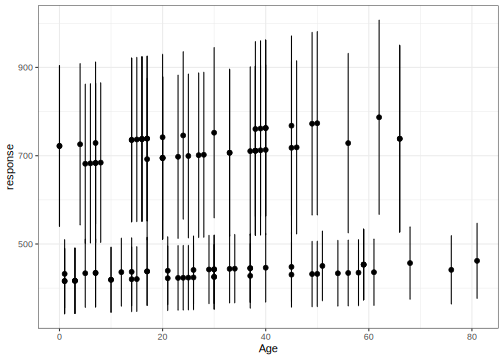
\includegraphics{0muestra_files/figure-beamer/unnamed-chunk-14-1.pdf}
\end{frame}

\begin{frame}[fragile]{Práctica en \texttt{R}}
\protect\hypertarget{pruxe1ctica-en-r-14}{}
\begin{Shaded}
\begin{Highlighting}[]
\FunctionTok{plot}\NormalTok{(encuesta}\SpecialCharTok{$}\NormalTok{dk,encuesta}\SpecialCharTok{$}\NormalTok{wk)}
\end{Highlighting}
\end{Shaded}

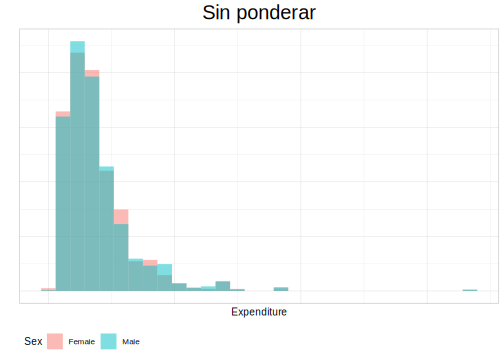
\includegraphics{0muestra_files/figure-beamer/unnamed-chunk-15-1.pdf}
\end{frame}

\begin{frame}[fragile]{Práctica en \texttt{R}}
\protect\hypertarget{pruxe1ctica-en-r-15}{}
\begin{Shaded}
\begin{Highlighting}[]
\FunctionTok{boxplot}\NormalTok{(encuesta}\SpecialCharTok{$}\NormalTok{wk }\SpecialCharTok{\textasciitilde{}}\NormalTok{ encuesta}\SpecialCharTok{$}\NormalTok{Stratum)}
\end{Highlighting}
\end{Shaded}

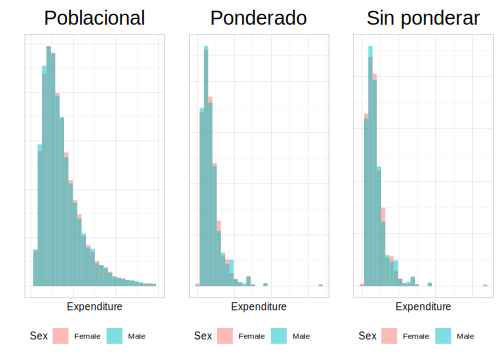
\includegraphics{0muestra_files/figure-beamer/unnamed-chunk-16-1.pdf}
\end{frame}

\begin{frame}[fragile]{Práctica en \texttt{R}}
\protect\hypertarget{pruxe1ctica-en-r-16}{}
\begin{Shaded}
\begin{Highlighting}[]
\FunctionTok{saveRDS}\NormalTok{(}\AttributeTok{object =}\NormalTok{ encuesta, }\AttributeTok{file =} \StringTok{"../Data/encuesta.rds"}\NormalTok{)}
\end{Highlighting}
\end{Shaded}
\end{frame}

\end{document}
